\subsection{要求仕様化}

要求仕様化とは、要求を記録し、記憶し、伝達できる形にする活動である。仕様化の方法は一つではない。自然言語で書く、構造化したテンプレートで書く、受け入れ基準として書く、モデルで表すなど、複数の方法がある。

どの方法を選ぶかは、プロジェクトの性質によって変わる。業務領域への理解、リスクの大きさ、チームの地理的分散、外注の有無、契約上の要求、要求に基づくテストの必要性、保守期間中の担当者交代などを考慮する必要がある。

\MiniBox{基本方針}{要求仕様は、読む人を意識して作る。利用者、顧客、設計者、開発者、テスト担当、保守担当は、それぞれ必要とする情報が違う。}

\subsubsection{非構造化自然言語による要求仕様化}

\term{非構造化自然言語}{Unstructured Natural Language}とは、通常の文章で要求を書く方法である。たとえば「システムは、利用者が注文履歴を検索できるようにする」といった文である。

利点は、誰でも読み書きしやすいことである。欠点は、曖昧さや抜け漏れが発生しやすいことである。自然言語は柔軟であるため、同じ文が複数の意味に読めることがある。

\subsubsection{構造化自然言語による要求仕様化}

\term{構造化自然言語}{Structured Natural Language}とは、自然言語を使いながら、書き方に制約を加える方法である。代表例は、\term{主体・動作形式}{Subject-Action Form}である。「いつ」「誰が」「何をする」「どの条件で」という形にそろえると、曖昧さを減らせる。

\MiniBox{例}{「注文が出荷されたとき、システムは請求書を作成する。ただし、注文条件が前払いの場合を除く。」この文では、きっかけ、主体、動作、例外条件が明示されている。}

他にも、\term{ユースケース仕様}{Use Case Specification}、\term{ユーザーストーリー}{User Story}、\term{決定表}{Decision Table}などが構造化自然言語の例である。ユーザーストーリーは、「ある役割として、ある能力がほしい。なぜなら、ある便益を得たいからである」という形式で、利用者視点の価値を表す。

\subsubsection{受け入れ基準に基づく要求仕様化}

\term{受け入れ基準}{Acceptance Criteria}とは、要求が満たされたと判断するための条件である。要求を受け入れ基準の形で書くと、テストと要求が強く結びつく。

\term{受け入れテスト駆動開発}{Acceptance Test-Driven Development}（ATDD）は、機能を作る前に、その機能が完成したと判断するテストを合意する方法である。\term{振る舞い駆動開発}{Behavior-Driven Development}（BDD）は、利用者の振る舞いを「前提、事象、結果」の形で書く方法である。

\MiniBox{BDDの例}{前提：口座残高が500円で、カードが有効である。事象：利用者が100円の出金を要求する。結果：ATMは100円を払い出し、口座残高は400円になる。}

この方法は、曖昧さの低減に有効である。一方で、どのシナリオを書くべきかを見落とすと不完全性は残る。そのため、境界値分析、組合せテスト、同値分割などのテスト技法と組み合わせるとよい。

\subsubsection{モデルに基づく要求仕様化}

\term{モデル}{Model}とは、複雑な対象を理解しやすくするために、必要な部分だけを抽象化して表したものです。要求仕様化では、文章だけでなく、図や形式的な記法を使って要求を表すことがある。UMLやSysMLの一部は、そのために使われる。

モデルは大きく二種類に分けられる。\term{構造モデル}{Structural Model}は、概念、データ、関係、業務規則を表す。\term{振る舞いモデル}{Behavioral Model}は、処理の流れ、利用者とのやり取り、状態遷移、イベントへの反応を表す。

\par\smallskip\noindent\refstepcounter{table}\label{tab:ch01-10}表 \thetable: モデルに基づく要求仕様化におけるモデルの種類・例\par\smallskip
表 \thetable は、モデルに基づく要求仕様化におけるモデルの種類・例を比較・確認しやすい形で整理したものである。\par\smallskip
\begin{tabularx}{0.97\linewidth}{@{}p{.24\linewidth}X@{}}
\toprule
\term{モデルの種類}{Types of Models} & 例 \\
\midrule
構造モデル & クラス図、概念データモデル、実体関連図。 \\
振る舞いモデル & ユースケース図、シーケンス図、状態遷移図、活動図、データフロー図。 \\
\bottomrule
\end{tabularx}

モデルには、手描きのラフな図から、数学的意味を厳密に持つ形式モデルまで幅がある。形式性が高いほど曖昧さは減るが、作成と理解の負担は増える。

\par\smallskip
\begin{center}
\centering
\IfFileExists{assets/generated_figures/ch01/fig-ch01-08.png}{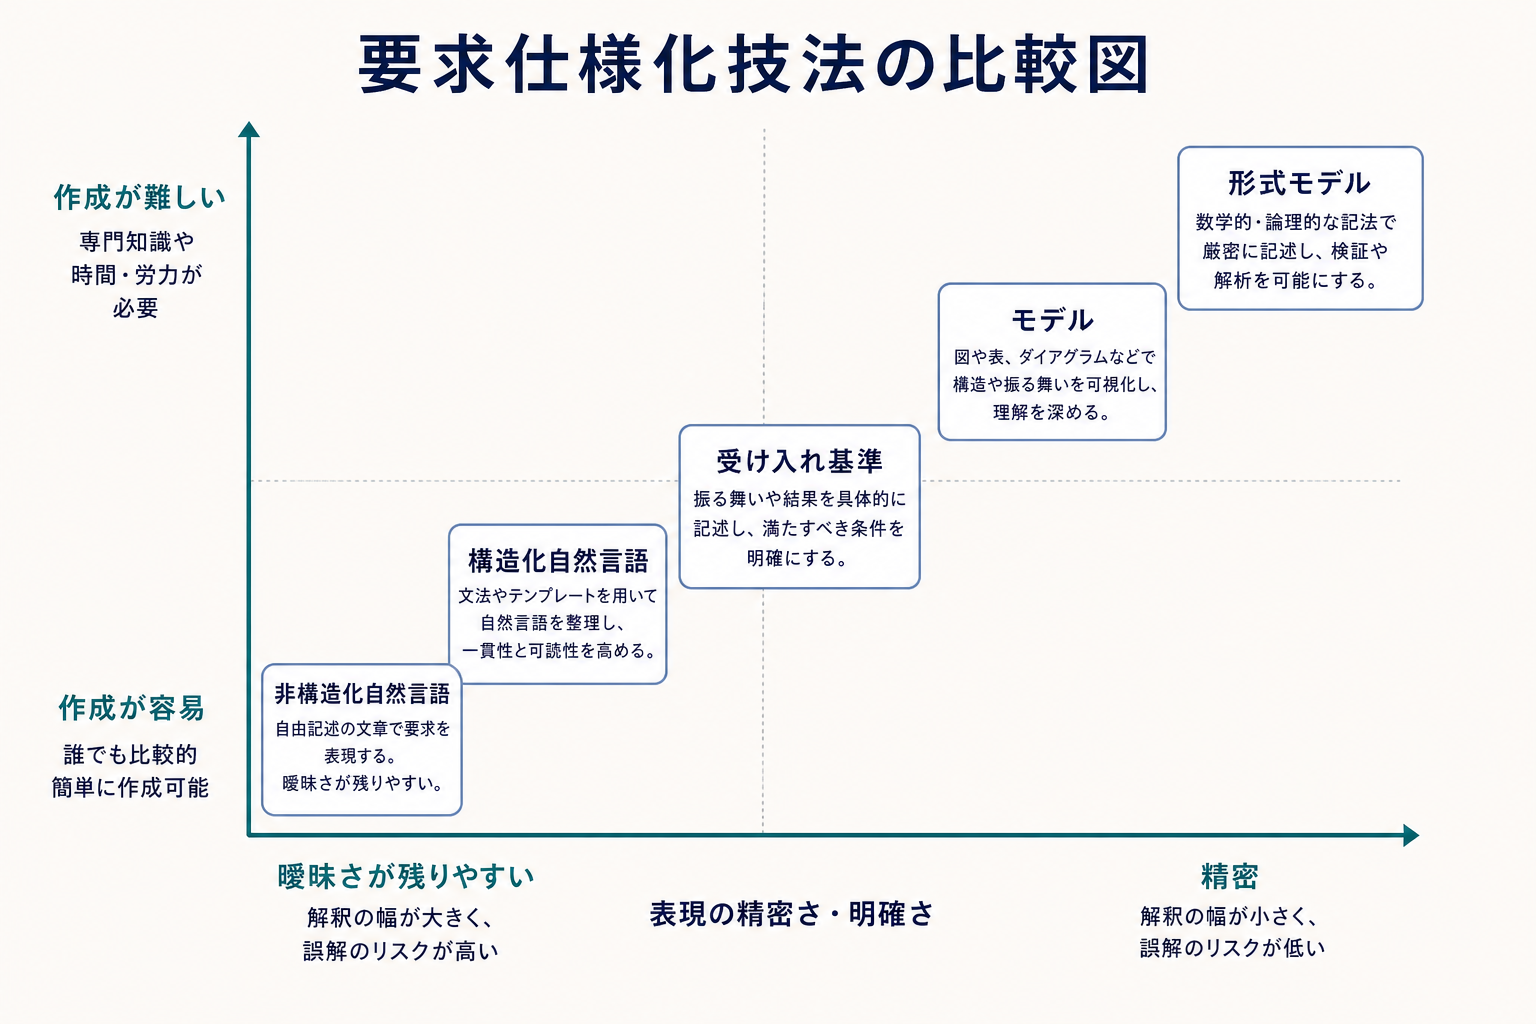
\includegraphics[width=0.96\linewidth]{assets/generated_figures/ch01/fig-ch01-08.png}}{\fbox{\parbox[c][48mm][c]{0.9\linewidth}{\centering 画像生成待ち\\要求仕様化技法の比較図}}}
\par\smallskip
\refstepcounter{figure}\label{fig:ch01-08}図 \thefigure: 要求仕様化技法の比較図
\end{center}
図 \thefigure は、要求仕様化技法の比較図を視覚的に整理したものである。
\par\smallskip

\subsubsection{要求の追加属性}

要求文そのものに加えて、要求を管理するための属性を付けると有用である。

\par\smallskip\noindent\refstepcounter{table}\label{tab:ch01-11}表 \thetable: 要求の追加属性における属性・目的\par\smallskip
表 \thetable は、要求の追加属性における属性・目的を比較・確認しやすい形で整理したものである。\par\smallskip
\begin{tabularx}{0.97\linewidth}{@{}p{.25\linewidth}X@{}}
\toprule
属性 & 目的 \\
\midrule
識別子 & 要求を一意に参照し、追跡する。 \\
説明 & 要求文だけでは足りない背景を補足する。 \\
根拠 & なぜその要求が必要かを説明する。 \\
源泉 & 誰または何から出た要求かを示す。 \\
種類 & 機能要求、技術制約、サービス品質制約などを示す。 \\
依存関係 & 他の要求との前後関係や依存を示す。 \\
衝突 & 他の要求と矛盾する可能性を示す。 \\
受け入れ基準 & 完了判定に使う条件を示す。 \\
優先度 & 重要度や実施順序を示す。 \\
安定性 & 変更される可能性を示す。 \\
変更履歴 & いつ、誰が、なぜ変更したかを残す。 \\
\bottomrule
\end{tabularx}

\subsubsection{増分的仕様化と包括的仕様化}

要求を明示的に文書化するプロジェクトでは、\term{増分的仕様化}{Incremental Specification}と\term{包括的仕様化}{Comprehensive Specification}の二つの考え方がある。

増分的仕様化では、今回の版で追加・変更・削除された差分だけを記録する。文書量は小さくなりやすいが、全体像を理解するには過去の差分を追う必要がある。

包括的仕様化では、各版にすべての要求を含める。文書量は増えるが、その版だけで全体を理解できる。実務では、マイナー版は差分、メジャー版は包括的に書くという組合せもある。
